\documentclass{beamer}
\usepackage{graphicx}
\usepackage{verbatim}
\usepackage{pifont}
\mode<presentation>
\title{JIT compilation for packet filtering using Netmap and LLVM}
\author[Peyrol\'on \and Chisnall]{Daniel Peyrol\'on \\ David Chisnall}
\date{Sep 16, 2014}
\setbeamertemplate{navigation symbols}{}

\begin{document}
\begin{frame}
  \titlepage
\end{frame}

\begin{frame}{Purpose of the project}
	\begin{itemize}
		\item \Large{This is a GSoC project for FreeBSD.}
		\item Development effort.
		\item Leverage Netmap for quick packet filtering.
	\end{itemize}
\end{frame}

\begin{frame}{Netmap}{}
	\begin{block}{}
		\begin{itemize}
			\item \Large{Kernel module.}
			\item Maps NIC rings with userspace.
			\item Userspace network stack.
			\item High speed for network operations.
		\end{itemize}
	\end{block}
\end{frame}

\begin{frame}{LLVM}{}
	\begin{block}{}
		\begin{itemize}
			\item \Large{Compiler framework.}
			\item Program compilation, analysis and transformation.
			\item Widely used.
		\end{itemize}
	\end{block}
\end{frame}

\begin{frame}{How does it work?}
	\begin{itemize}

		\item \Large{How rules are interpreted.}
		\begin{itemize}
			\item \Large{Example: \textit{''accept tcp from any to any 80''}}
		\end{itemize}

		\item How the JIT works.
		\begin{itemize}
			\item \Large{Loads external LLVM bitcode.}
			\item Bitcode contains functions and structs used.
			\item Functions called from the JIT, inlined.
			\item Iterate through the ruleset and emit code.
		\end{itemize}

	\end{itemize}
\end{frame}

\begin{frame}{Compilation}
	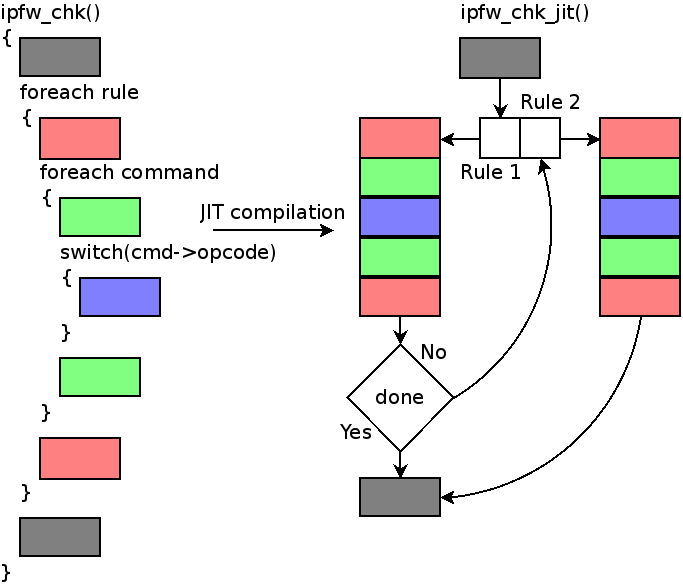
\includegraphics[height=0.8\textheight, width=0.8\textwidth]{Figure1}
\end{frame}

\begin{frame}[fragile]{Benefits from this approach}
	\begin{itemize}
		\item \Large{It's easy to develop and update the compiler.}
		\item General solution for packet filtering.
	\end{itemize}
	\large
	\begin{block}{}
		\begin{verbatim}
		 case O_ACCEPT:
		    rule_accept(&retval, &l, &done );
		    break;
		\end{verbatim}
		\begin{verbatim}
		emit_accept(){
		    Irb.CreateCall(RuleAccept, {Retval, L, Done});
		}
		\end{verbatim}
	\end{block}
\end{frame}

\begin{frame}{Basic benchmarking}
	\Large
	\begin{center}
		Basic benchmark for 1k pkts
		\begin{tabular}{|c|c|c|}
			\hline
			JIT compiler & Compilation & 130ms \\ \cline{2-3}
			& Filtering & \textbf{523 $\mu$s} \\
			\hline
			Interpreter & Filtering & 3664 $\mu$s \\
			\hline
		\end{tabular} \\
		Speedup = x7 for filtering code \\
		Compilation time $\equiv$ Interpreting rules for 35480 pkts \\
		Packets needed for amortization $\equiv$ 41440 pkts \\
	\end{center}
\end{frame}

\begin{frame}{Future work}
	\begin{itemize}
		\item \Large{Complete the firewall.}
		\item Benchmarking, evaluation.
		\item Static analysis.
		\item Feedback-driven optimisations.
	\end{itemize}
\end{frame}

\begin{frame}{What I'm trying to say}
	\begin{itemize}
		\item \Large{It works!}
		\item Perhaps it's interesting for someone?
		\item Ongoing development effort.
		\item Thanks to many people.
	\end{itemize}
\end{frame}

\begin{frame}
	\title{Thanks for your attention! \\ \vspace{30pt} Questions? \\ Suggestions?}
	\date{}
	\author[]{}
	\titlepage
\end{frame}

\end{document}
